\vspace{-10ex}%
\rule{\textwidth}{0.3pt}
\vspace{10ex}
 % after-code

This chapter will guid the reader through the whole process of developing a system prototype. Designing the PCB, soldering the components, troubleshooting the board and writing the neccesary code are some of the steps involved and they will all be described in detail here.

\section{Schematics}
The schematics over the circuit is created by placing all the components discussed earlier, every IC have a small amont of components that is placed in a way so that it is easy to understand which components is belongs to which. A title is added to every part in the design for a good overwiev over the system. Since the section which included the radio is large it is placed on a separate page. When additional components are added in additional pages can be inserded. These schematics can be found in "aoutoref appendix schematics".

\section{Layout} 
\subsection{First design} The first of two boards is 3.5 times 3.5 mm in size. The different parts of the circuit is layed out in a way that it is easy to inspect and resolder if neccesary. The main components of the board is placed close to each other at one side to get an idea of the design for the final product. This board is equipped with some testpoints for easy connections with test probes and oscillioscope. The silcskreen print on the top of the board was vague at some places and made destinguish them between eachother hard. The pin one location at one part could not been spottet.  A view of the board can be seen in \autoref{PCB_rev1}. 

\begin{figure}[H]
	\centering
    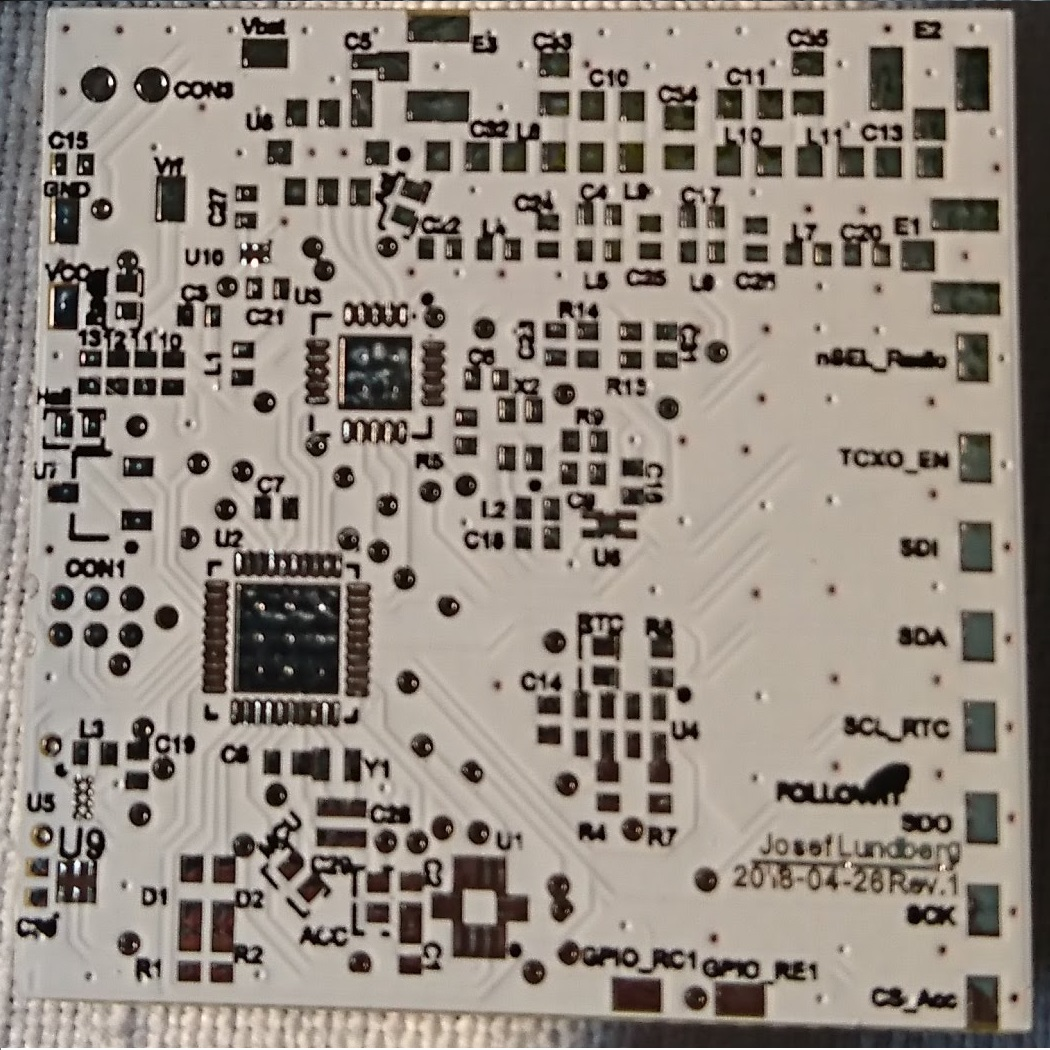
\includegraphics[width=.8\linewidth]{Figures/PWB}
	\captionsource{First (1) revision circuit board.}{Author}
	\label{fig:pcbr1}
\end{figure}


% Kanske inte
\section{Power consumption}
When running the processor at operation speed and voltage the 
The power consumption is first mesured with only the processor connected. 